\documentclass[aspectratio=169]{beamer}

\usetheme{Madrid}
\usecolortheme{seahorse}

\usepackage{amsmath}
\usepackage{amssymb}
\usepackage{booktabs}
\usepackage{graphicx}
\usepackage{mathtools}

\graphicspath{{plots/}{../plots/}}

\title[Power Allocation]{Design and Evaluation of Machine Learning Frameworks for Proportional Fairness Power and Resource Allocation in Multi-User Wireless Networks}
\author{Sai Rithvik Achutuni}
\date{\today}

\newcommand{\Rbar}{\overline{R}}
\newcommand{\SINR}{\operatorname{SINR}}

\begin{document}

\begin{frame}
  \titlepage
\end{frame}

\section{Introduction}

\begin{frame}{Challenge in next gen networks}
    \begin{figure}
        \centering
        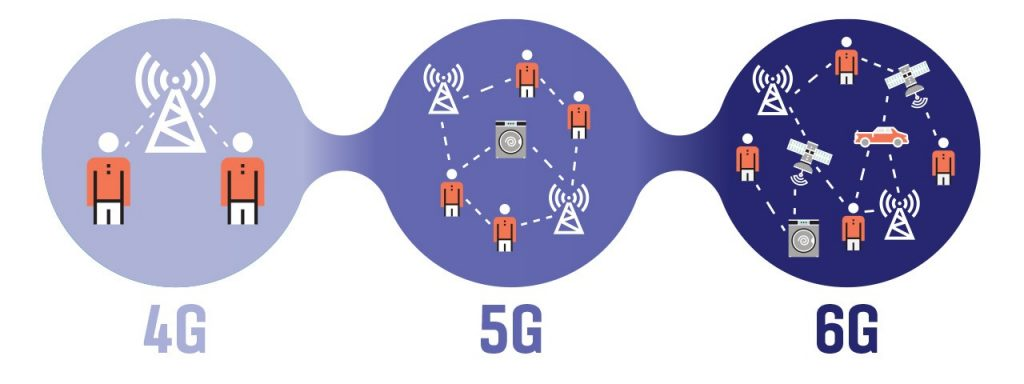
\includegraphics[height=0.2\textheight]{image.jpg}
    \end{figure}
    Modern network architectures are mandated to accommodate an exponentially growing density of heterogeneous devices while delivering ultra-reliable, low-latency connectivity.
    \newline
    \newline
    The performance benchmarks established for 6G target peak data rates of 1.0 terabits per second and air-interface latencies approaching 0.1 milliseconds, figures that vastly exceed the capabilities of legacy cellular infrastructures
    
\end{frame}

\begin{frame}{The core problem}
    Dynamically allocating limited radio resources—specifically, an allocation across $K$ shared orthogonal frequency resources and a finite total transmit power budget $P$ —among $N$ competing client devices in a multi-user environment.
    \newline
    \newline
    The problem of choosing transmit power dynamically in response to physical channel conditions in order to
    maximize the downlink sum-rate with maximal power constraints is NP-hard.\cite{plch}
\end{frame}

\begin{frame}{Limits of Traditional Methods}
    \begin{itemize}
        \item computational complexity
        \item traditional models fail to account for hardware and channel imperfections
        \item specific hardware components such as low-resolution A/D, nonlinear amplifier are challenging to be developed. \cite{rybicka}
    \end{itemize}
\end{frame}

\section{System Model}

\begin{frame}{System Model}
    \begin{itemize}
            \item The environment consists of a base station serving $N$ active clients.
        \item Clients compete for $K$ orthogonal frequency resources.
        \item $\mathbf{P}_{n,k}$: Continuous transmit power allocated to client $n$ on resource $k$.
        \item \textbf{Sum-Power Constraint:} Total aggregate power is limited by a physical budget $P_{total}$.
        \begin{equation*}
        \sum_{n=1}^{N} \sum_{k=1}^{K} P_{n,k} \le P_{total} \quad
        \end{equation*}
    \end{itemize}
\end{frame}

\begin{frame}{The Wireless Environment: Interference \& Capacity}
    \begin{itemize}
        \item \textbf{SINR Formulation:} The Signal-to-Interference-plus-Noise Ratio ($\gamma_{n,k}$) for client $n$ on resource $k$ accounts for co-channel interference:
        $$\gamma_{n,k} = \frac{p_{n,k} |h_{n,k}|^2}{\sum_{j \neq n} p_{j,k} |h_{n,j}|^2 + \sigma^2}$$
        \item \textbf{Achievable Data Rate:} According to the Shannon-Hartley theorem, the data rate $r_{n,k}$ given bandwidth $B$ is:
        $$r_{n,k} = B \log_2(1 + \gamma_{n,k})$$
        \item \textbf{Aggregate Throughput:} The instantaneous total rate for client $n$ is $R_n = \sum_{k=1}^K r_{n,k}$.
    \end{itemize}
\end{frame}

\begin{frame}{The Trade-Off: Throughput vs. Fairness}
    \begin{itemize}
        \item \textbf{The Core Conflict:} Designing a scheduler to maximize total network throughput (sum-rate) inherently favors users with optimal, unobstructed channel conditions.
        \item \textbf{Cell-Edge Starvation:} Exclusively prioritizing these strong channels leads to the severe resource deprivation or "starvation" of cell-edge users who experience high path loss and interference.
        \item \textbf{Enforcing Equity:} Maintaining fairness requires the network to actively allocate finite resources to users with poorer channel conditions, guaranteeing a baseline quality of service for everyone.
    \end{itemize}
\end{frame}

\begin{frame}{The $\alpha$-Fairness Utility Paradigm}
    \begin{itemize}
        \item \textbf{Objective:} Maximize overarching network utility $U_\alpha(\mathbf{R})$ to navigate the throughput versus fairness trade-off.
        \item \textbf{Mathematical Framework:}
        $$U_\alpha(\mathbf{R}) = \begin{cases} \sum_{n=1}^N \frac{R_n^{1-\alpha}}{1-\alpha}, & \text{if } \alpha \ge 0, \alpha \neq 1 \\ \sum_{n=1}^N \log(R_n), & \text{if } \alpha = 1 \end{cases}$$
        \item \textbf{Operational Behaviors:}
        \begin{itemize}
            \item $\alpha=0$: Sum-Rate Maximization (favors strong channels, risks edge-user starvation).
            \item $\alpha=1$: Proportional Fairness (maximizes geometric mean of user rates).
            \item $\alpha\to\infty$: Max-Min Fairness (guarantees absolute equity but severely penalizes capacity).
        \end{itemize}
    \end{itemize}
\end{frame}

\section{literature review}

\begin{frame}
    \huge
    \centering
    Literature Review
\end{frame}

\begin{frame}{Deep Unrolling}
    \begin{itemize}
        \item \textbf{Core Concept:} Deep unrolling converts classical iterative optimization algorithms into deep neural networks by mapping each iteration directly to a network layer.\cite{He2022}
        \item \textbf{Mathematical Rigor:} This approach blends the structural insights of proven iterative algorithms with the adaptive learning capabilities of neural networks, offering superior interpretability over generic models.
        \item \textbf{Constraint Satisfaction:} Frameworks can utilize projection gradient descent during forward passes to strictly enforce complex, non-convex constraints, such as total power budgets.
    \end{itemize}
\end{frame}

\begin{frame}{Deep Reinforcement Learning (DRL)}
    \begin{itemize}
        \item \textbf{Model-Free Optimization:} DRL techniques offer a model-free alternative for navigating NP-hard wireless resource allocation problems by learning directly from environmental interactions.
        \item \textbf{Algorithm Selection:} Advanced frameworks frequently utilize Proximal Policy Optimization (PPO) for user scheduling tasks, while algorithms like Deep Deterministic Policy Gradient (DDPG) handle continuous power allocation.
        \item \textbf{Action Space Management:} To combat the curse of dimensionality in large networks, modern models integrate K-Nearest Neighbors (KNN) clustering to efficiently discretize continuous action spaces.
    \end{itemize}
\end{frame}

\begin{frame}{Enforcing Proportional Fairness in DRL}
    \begin{itemize}
        \item \textbf{Fairness Formulations:} Proportional fairness can be mathematically embedded into the DRL objective by maximizing the logarithmic utility $\beta(z) = \log(z)$ of user data rates.
        \item \textbf{Dynamic Weighting:} Advanced DRL schedulers prevent cell-edge user starvation by dynamically applying scheduling weights based on historical throughput, actively punishing policies that leave users underserved.
        \item \textbf{Reward Penalization:} Agents can be trained with strict reward penalization, receiving zero rewards if their proposed continuous allocation violates predetermined Service Level Agreements.
    \end{itemize}
\end{frame}

\section{My Implementation}
\begin{frame}
    \huge
    \centering
    My implementation
\end{frame}

\begin{frame}{Shared Wireless System Model}
  The implementation studies an $N$-user interference channel with complex channel matrix $H$ and power vector $p$.

  \begin{align*}
    \SINR_k(p, H)
      &= \frac{|H_{k,k}|^2 p_k}
              {\sum_{j \ne k}|H_{k,j}|^2 p_j + \sigma^2}, \\
    R_k(p, H)
      &= B \log_2\left(1 + \SINR_k(p, H)\right), \\
    \sum_{k=1}^{N} p_k &\le P_{\max}, \qquad p_k \ge 0.
  \end{align*}

  \vspace{0.5em}
  \begin{itemize}
    \item Implemented in \texttt{src/performance.py} and reused by evaluation scripts.
    \item Baselines solve different tradeoffs between sum-rate and fairness.
    \item Water filling is implemented in code but excluded here.
  \end{itemize}
\end{frame}

\begin{frame}{Dynamic CSI Transition}
  \texttt{WirelessAllocationEnv} and \texttt{DynamicChannelSimulator} model mobile fading with a first-order Gauss-Markov process:

  \[
    H_{t+1}
      = \rho H_t + \sqrt{1-\rho^2}E_t,
      \qquad
      E_t \sim \mathcal{CN}(0,1).
  \]

  The correlation coefficient follows Jakes' model:

  \[
    \rho = J_0(2\pi f_d T_{\mathrm{TTI}}),
    \qquad
    f_d = \frac{v}{\lambda}.
  \]

  \begin{itemize}
    \item Carrier frequency: $2$ GHz.
    \item Mobility setting in evaluations: $60$ km/h.
  \end{itemize}
\end{frame}

\begin{frame}{Baseline 1: Fractional Programming}
  targets sum-rate maximization:

  \begin{align*}
    \max_{p \ge 0}\quad
      &\sum_{k=1}^{N}\log\left(1 +
        \frac{G_{k,k}p_k}{\sum_{j \ne k}G_{k,j}p_j + \sigma^2}\right) \\
    \text{s.t.}\quad
      &\sum_{k=1}^{N}p_k \le P_{\max},
      \qquad G_{k,j}=|H_{k,j}|^2.
  \end{align*}

  The code uses a quadratic-transform style auxiliary variable:

  \[
    y_k =
    \frac{\sqrt{G_{k,k}p_k}}
         {\sum_{j \ne k}G_{k,j}p_j + \sigma^2 + G_{k,k}p_k}.
  \]

  Power is updated by gradient ascent, clipped to nonnegative values, and projected back to the total power budget.
\end{frame}

\begin{frame}{Baseline 2: Proportional-Fair WMMSE}
  weighted WMMSE with proportional-fair weights:

  \[
    \alpha_k = \frac{1}{\Rbar_k + \epsilon}.
  \]

  With $v_k=\sqrt{p_k}$, each iteration updates receiver filters, MSE weights, and transmit amplitudes:

  \begin{align*}
    u_k &=
    \frac{H_{k,k}v_k}
         {\sum_j |H_{k,j}|^2 v_j^2 + \sigma^2}, \\
    e_k &=
    1 - 2\Re(u_k H_{k,k}v_k)
      + |u_k|^2\left(\sum_j |H_{k,j}|^2 v_j^2 + \sigma^2\right), \\
    w_k &= \frac{\alpha_k}{\max(e_k, 10^{-9})}.
  \end{align*}

  The transmit update uses KKT bisection to find $\mu$ so that $\sum_k v_k^2 \le P_{\max}$.
\end{frame}

\begin{frame}{Baseline 3: Max-Min Fairness}
  \texttt{max\_min\_power\_allocation} searches for the largest common SINR target $\gamma$ that all users can satisfy:

  \begin{align*}
    \max_{p,\gamma}\quad &\gamma \\
    \text{s.t.}\quad
      &\frac{G_{k,k}p_k}{\sum_{j \ne k}G_{k,j}p_j + \sigma^2} \ge \gamma,
      \quad \forall k, \\
      &\sum_k p_k \le P_{\max}, \qquad p_k \ge 0.
  \end{align*}

  For a fixed target $\gamma$, the required powers solve:

  \[
    \left(I - \gamma D^{-1}F\right)p
      = \gamma D^{-1}\sigma^2\mathbf{1}.
  \]

  The implementation performs bisection over $\gamma$ and keeps the highest feasible power vector.
\end{frame}

\begin{frame}{Motivation: Why PPO?}
    \begin{itemize}
        \item \textbf{Stability:} Standard Policy Gradients are sensitive to step sizes.
        \item \textbf{Simplicity:} PPO achieves the stability of TRPO but uses only first-order optimization.
        \item \textbf{Efficiency:} Better sample complexity than REINFORCE or A2C.
    \end{itemize}
    \begin{block}{The Goal}
        Maximize performance while ensuring the new policy doesn't deviate too far from the old policy.
    \end{block}
\end{frame}

% Slide 3: The Clipped Objective
\begin{frame}{The Clipped Surrogate Objective}
    The core of PPO is the clipped objective function:
    \begin{equation*}
        L^{CLIP}(\theta) = \hat{\mathbb{E}}_t \left[ \min(r_t(\theta)\hat{A}_t, \text{clip}(r_t(\theta), 1-\epsilon, 1+\epsilon)\hat{A}_t) \right]
    \end{equation*}
    
    Where:
    \begin{itemize}
        \item $r_t(\theta) = \frac{\pi_\theta(a_t|s_t)}{\pi_{\theta_{old}}(a_t|s_t)}$ is the probability ratio.
        \item $\hat{A}_t$ is the estimated advantage.
        \item $\epsilon$ is a hyperparameter (typically 0.1 or 0.2).
    \end{itemize}
\end{frame}

\begin{frame}{PPO: MDP Formulation}
  The DRL agent treats power allocation as an MDP
  $(\mathcal{S}, \mathcal{A}, \mathcal{P}, \mathcal{R}, \gamma)$.

  \begin{block}{State}
    \[
      s_t =
      \left[
        \operatorname{vec}(|H_t|),
        \frac{\Rbar_t}{10B}
      \right]
      \in \mathbb{R}^{N^2 + N}.
    \]
  \end{block}

  \begin{block}{Action}
    \[
      a_t \in [0,1]^N,
      \qquad
      p_t = P_{\max}a_t.
    \]
  \end{block}

  The state includes both instantaneous CSI and historical throughput so the policy can learn channel-aware and fairness-aware decisions.
\end{frame}

\begin{frame}{PPO: Reward and Feasibility}
  The environment uses logarithmic utility to encode proportional fairness:

  \[
    r_t =
      \sum_{k=1}^{N}\log(R_{k,t}+\epsilon)
      - 5\max\left(0, \sum_k p_{k,t} - P_{\max}\right).
  \]

  If the action exceeds the hardware budget, powers are projected back:

  \[
    p_t \leftarrow
      p_t \frac{P_{\max}}{\sum_k p_{k,t}}
      \quad \text{when } \sum_k p_{k,t} > P_{\max}.
  \]

  Historical rates are updated with an exponential moving average:

  \[
    \Rbar_{k,t+1}=0.8\Rbar_{k,t}+0.2R_{k,t}.
  \]
\end{frame}



\begin{frame}{PPO: Policy Optimization}
  The training script uses Stable-Baselines3 PPO with an MLP policy.

  PPO optimizes a clipped policy-gradient objective:

  \[
    L^{\mathrm{CLIP}}(\theta)
      =
      \mathbb{E}_t
      \left[
        \min\left(
          r_t(\theta)\hat{A}_t,
          \operatorname{clip}(r_t(\theta), 1-\epsilon, 1+\epsilon)\hat{A}_t
        \right)
      \right],
  \]

  where

  \[
    r_t(\theta)
      =
      \frac{\pi_\theta(a_t|s_t)}
           {\pi_{\theta_{\mathrm{old}}}(a_t|s_t)}.
  \]

  Clipping limits destructive policy updates while still allowing continuous power vectors.
\end{frame}

\begin{frame}{PPO: Training Pipeline}
  \begin{table}
    \centering
    \begin{tabular}{ll}
      \toprule
      Component & Implementation choice \\
      \midrule
      Environment & \texttt{WirelessAllocationEnv(num\_users=6, p\_max=10)} \\
      API validation & \texttt{check\_env(env, warn=True)} \\
      Policy & \texttt{PPO("MlpPolicy", env)} \\
      Learning rate & $3\times 10^{-4}$ \\
      Rollout length & $2048$ steps \\
      Batch size & $64$ \\
      Discount factor & $\gamma=0.99$ \\
      Training horizon & $200{,}000$ timesteps \\
      \bottomrule
    \end{tabular}
  \end{table}

  Separate saved models are used for $N \in \{3,4,5,6\}$ in the scaling evaluations.
\end{frame}


\begin{frame}{Results: Average Sum-Rate}
  \centering
  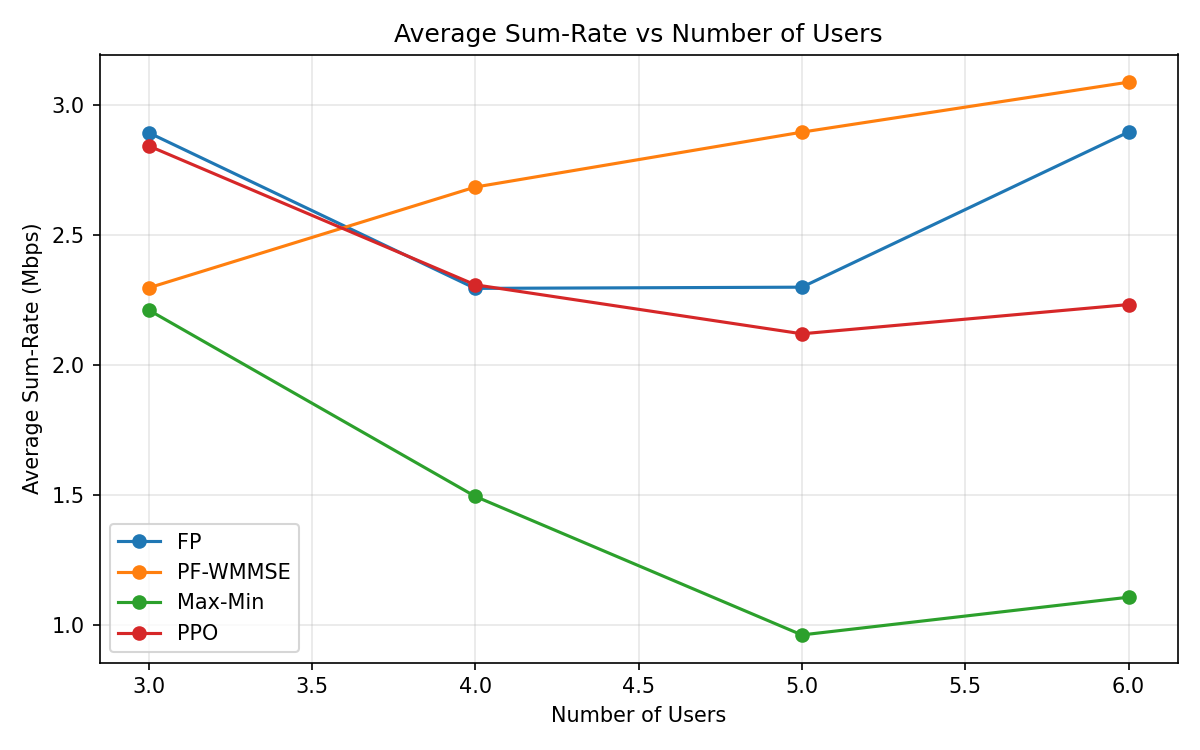
\includegraphics[height=0.58\textheight]{sum_rate_vs_users.png}

  \vspace{0.5em}
  \small
  \begin{itemize}
    \item FP is the sum-rate-oriented upper reference and can sacrifice fairness.
    \item Max-min preserves equality but gives up total throughput.
    \item PPO is evaluated as a learned proportional-fair policy against PF-WMMSE.
  \end{itemize}
\end{frame}

\begin{frame}{Results: Jain Fairness}
  \centering
  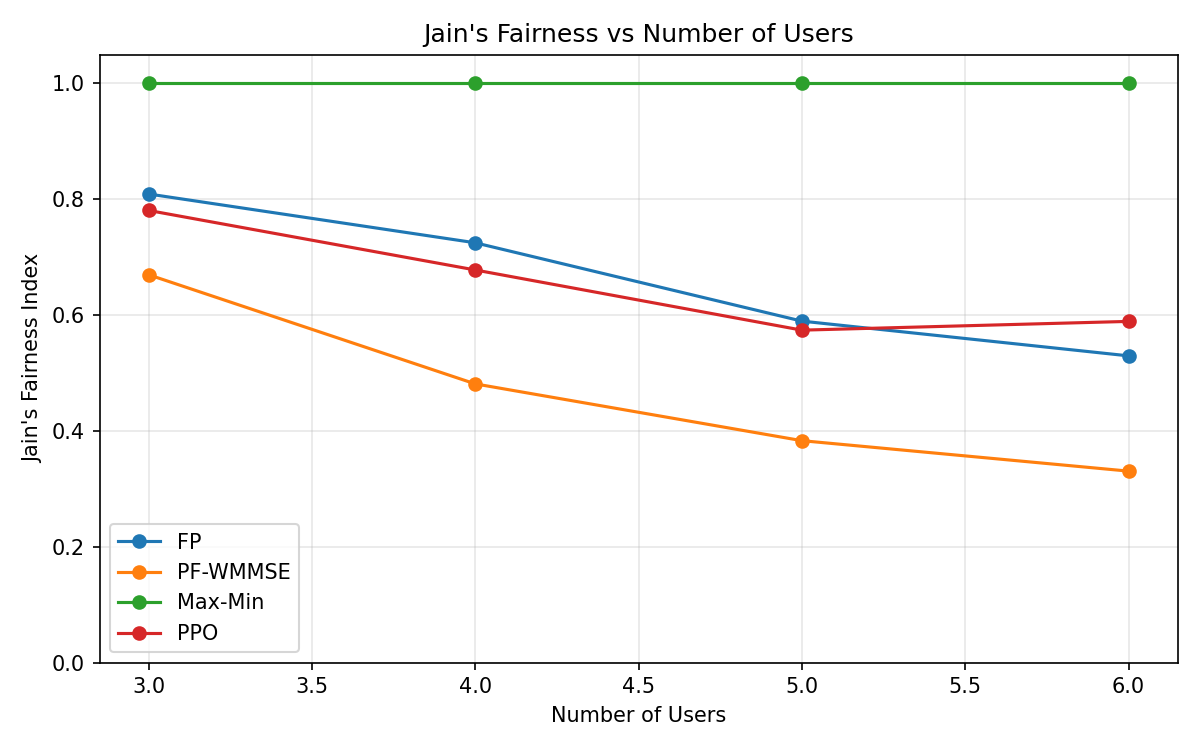
\includegraphics[height=0.55\textheight]{jain_fairness_vs_users.png}

  \vspace{0.5em}
  \small
  Jain's index is computed as
  \[
    J(R)=\frac{\left(\sum_k R_k\right)^2}{N\sum_k R_k^2}.
  \]

  PPO and PF-WMMSE are the relevant proportional-fair comparison because both include historical-rate feedback.
\end{frame}

\section{Whats Next?}



\begin{frame}{Results: Execution Time}
  \centering
  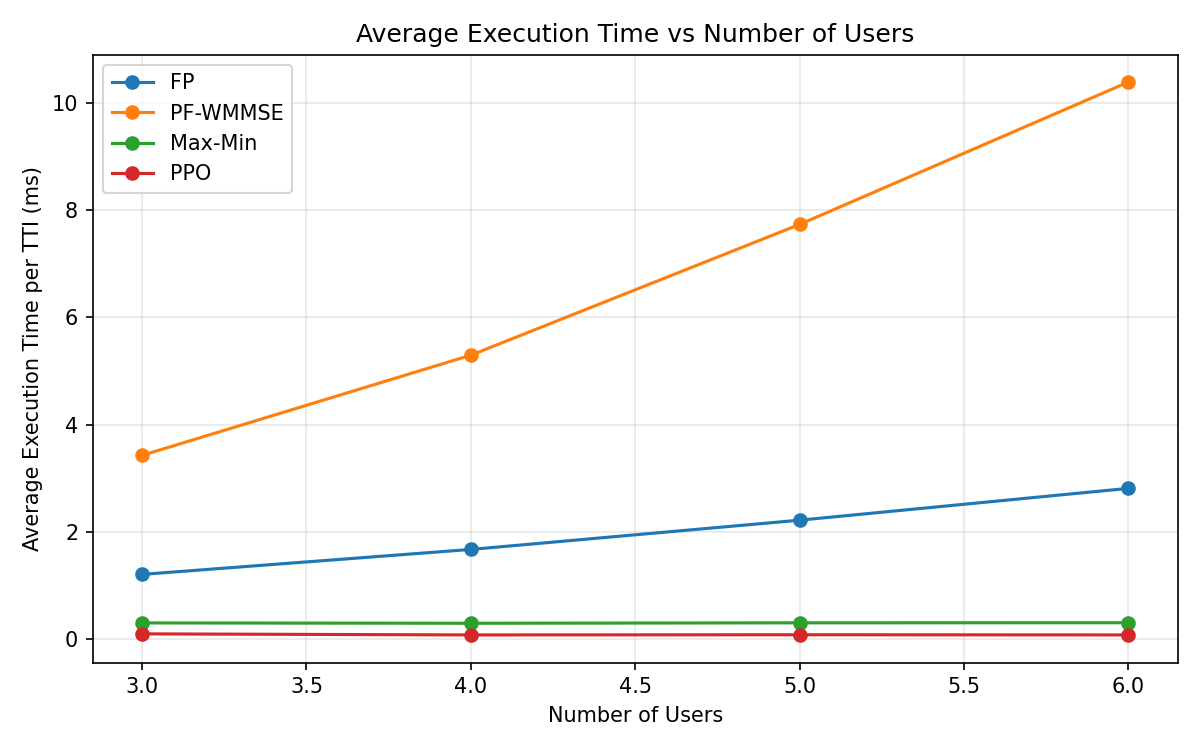
\includegraphics[height=0.58\textheight]{avg_time_vs_users.png}

  \vspace{0.5em}
  \small
  \begin{itemize}
    \item Classical baselines repeatedly solve iterative updates per TTI.
    \item PPO shifts most cost to offline training; online control is a deterministic forward pass.
    \item The implementation goal is not only high reward, but fast decisions under dynamic CSI.
  \end{itemize}
\end{frame}

\begin{frame}{Future Work}
  \begin{itemize}
    \item The current PPO implementation is a proof of concept and has not been extensively tuned for performance.
    \item More extensive simulations with larger user counts and different mobility settings are needed to fully evaluate scalability and robustness.
  \end{itemize}
\end{frame}

\begin{frame}{Major Drawbacks}
  The cuurrent implementation has several limitations:
  \begin{itemize}
    \item The PPO agent is trained on a single mobility setting (60 km/h) and may not generalize well to other speeds or fading conditions.
    \item The PPO agent must train separate models for each user count, which limits scalability and adaptability in real-world deployments where user counts can fluctuate.
  \end{itemize}
\end{frame}

\begin{frame}{Meta-Learning for Adaptability}
  To address the scalability and generalization issues, future work could explore meta-learning approaches that enable the PPO agent to quickly adapt to new user counts and mobility settings with minimal additional training.

  \begin{itemize}
    \item Meta-learning algorithms like MAML could be used to train a single model that can fine-tune efficiently to new conditions.
    \item This would allow the agent to maintain high performance across a wider range of scenarios without needing separate models for each configuration.
  \end{itemize}

\end{frame}

\begin{frame}{MAML: Learning to Learn}
    \begin{itemize}
        \item \textbf{Goal:} Train a model that can adapt to a new task with very few data points and a few gradient steps.
        \item \textbf{Key Idea:} Find an initialization $\theta$ such that the model is highly sensitive to the gradient updates of new tasks.
        \item \textbf{Agnostic:} Works with any model architecture that uses gradient descent.
    \end{itemize}
    \begin{block}{The Difference}
        Standard Transfer Learning learns a good feature extractor; MAML learns an \textbf{optimal starting point} for optimization.
    \end{block}
\end{frame}

% Slide 3: The Optimization
\begin{frame}{Bilevel Optimization Structure}
    For a task distribution $p(\mathcal{T})$, MAML updates parameters in two loops:
    
    \vspace{0.5cm}
    \textbf{1. Inner Loop (Task-Specific):}
    \begin{equation}
        \theta'_i = \theta - \alpha \nabla_\theta \mathcal{L}_{\mathcal{T}_i}(f_\theta)
    \end{equation}
    
    \textbf{2. Outer Loop (Meta-Update):}
    \begin{equation}
        \theta \leftarrow \theta - \beta \nabla_\theta \sum_{\mathcal{T}_i \sim p(\mathcal{T})} \mathcal{L}_{\mathcal{T}_i}(f_{\theta'_i})
    \end{equation}
    
    \textit{Note: The outer loop requires computing gradients through gradients (Hessian-vector products).}
\end{frame}

\section{Bibliography}
\begin{frame}{Bibliography}

\begin{thebibliography}{9}
\bibitem{plch}Z. Q. Luo and S. Zhang, “Dynamic spectrum management: Complexity and duality,” 

\bibitem{rybicka}Meng, Fan \& Chen, Peng \& Wu, Lenan \& Cheng, Julian. (2020). Power Allocation in Multi-User Cellular Networks: Deep Reinforcement Learning Approaches.

\bibitem{He2022} S. He et al., ``An Unsupervised Deep Unrolling Framework for Constrained Optimization Problems in Wireless Networks,'' \textit{IEEE Trans. Wireless Commun.}, 2022.[2]
\bibitem{Lopes2024} H. H. S. Lopes et al., ``Deep Deterministic Policy Gradient-Based Resource Allocation,'' \textit{Sensors}, 2024.[4]
\bibitem{Matemu2026} A. Matemu et al., ``Joint Scheduling and Power Allocation in O-RAN via PPO,'' \textit{TechRxiv}, 2026.[4]
\bibitem{Eisen2020} M. Eisen and A. Ribeiro, ``Optimal Wireless Resource Allocation With Random Edge Graph Neural Networks,'' \textit{IEEE Trans. Signal Process.}, 2020.[6]
\bibitem{Yang2024} H. Yang et al., ``Knowledge-Driven Resource Allocation: A WMMSE Unrolled GNN Approach,'' \textit{IEEE Internet of Things J.}, 2024.

\end{thebibliography}

\end{frame}


\end{document}
